\section{Les masses d'air et les fronts}
	\subsection{Les masses d'air}
		\subsubsection{Anticyclones}
		\subsubsection{Dépressions}
		\subsubsection{Cols, dorsales, talwegs et marais barométriques}
	\subsection{Les fronts}
	
		\begin{figure}[H]
			\centering
			\includegraphics[width=0.85\linewidth]{03-Meteo/img/frontIsobares20260127.png}
			\legende{Carte des isobares}{img:frontIsobares20260127}
		\end{figure}	
		
		\begin{figure}[H]
			\centering
			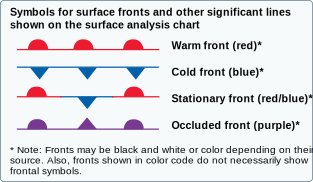
\includegraphics[width=0.4\linewidth]{03-Meteo/img/legendeFronts.pdf}
			\legende{Symboles des fronts sur une carte météorologique}{img:legendeFronts}
		\end{figure}	
	
	
		\subsubsection{Front froid}
		\begin{figure}[H]
			\centering
			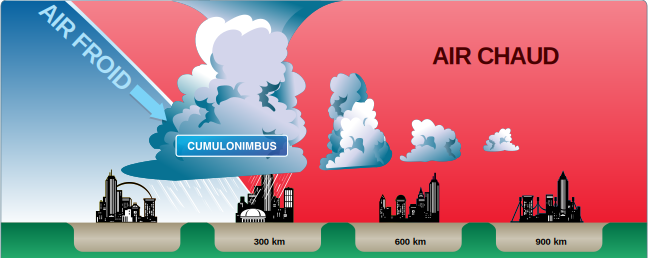
\includegraphics[width=0.75\linewidth]{03-Meteo/img/frontFroid.pdf}
			\legende{Coupe d'un front froid}{img:frontFroid}
		\end{figure}	
		
		
		\subsubsection{Front chaud}
		\begin{figure}[H]
			\centering
			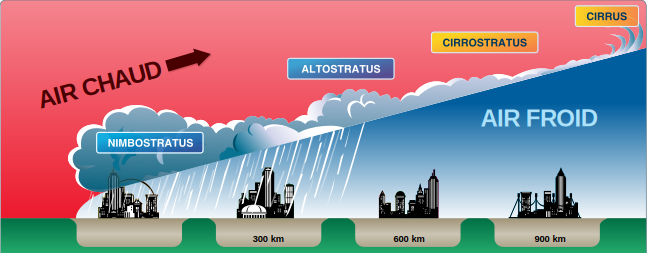
\includegraphics[width=0.75\linewidth]{03-Meteo/img/frontChaud.pdf}
			\legende{Coupe d'un front chaud}{img:frontChaud}
		\end{figure}	
		
		
		\subsubsection{Front occlus}
		\begin{figure}[H]
			\centering
			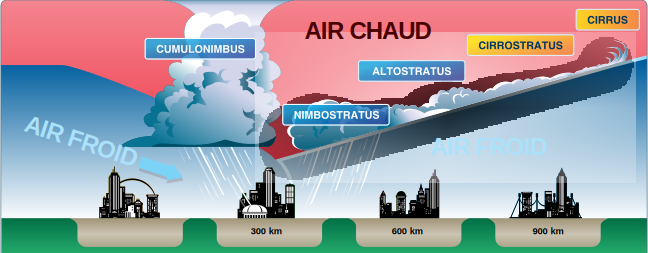
\includegraphics[width=0.75\linewidth]{03-Meteo/img/frontOcclus.pdf}
			\legende{Coupe d'un front occlus}{img:frontOcclus}
		\end{figure}		
		
		\subsubsection{Front quasi stationnaire}